\usepackage{etex} %эта магическая херь избавляет от переполнения регистров TeX а!!!

\mode<article>{\usepackage{fullpage}}
\mode<presentation>{
    \usetheme{Madrid}
    \useoutertheme{shadow}
} 

\usepackage[utf8]{inputenc}
\usepackage[russian]{babel}
\usepackage{indentfirst}
\usepackage{graphicx}

\usepackage{amsmath}
\usepackage{amsfonts}
\usepackage{amsthm}
%\usepackage{algorithm}
%\usepackage{algorithmic}

%\usepackage[all]{xy}

\date{Лекция по дисциплине <<методы и средства защиты компьютерной информации>> (\today)}
\author[М.~М.~Шихов]{Михаил Шихов \\ \texttt{\underline{m.m.shihov@gmail.com}}}

%%для рисования графов пакетом xy-pic
%\entrymodifiers={++[o][F-]}

%%для псевдокода алгоритмов (algorithm,algorithmic)
%\renewcommand{\algorithmicrequire}{\textbf{Вход:}}
%\renewcommand{\algorithmicensure}{\textbf{Выход:}}
%\renewcommand{\algorithmiccomment}[1]{// #1}
%\floatname{algorithm}{Псевдокод}

%\setbeamercolor{alerted text}{fg=-green} %gyan, blue, green, -green



\title[Угрозы, атаки]{Угрозы информационной безопасности}


\begin{document}


\mode<article>{\maketitle\tableofcontents}

\frame<presentation>{\titlepage}
\begin{frame}<presentation>[allowframebreaks]
\frametitle{Содержание}
\tableofcontents
\end{frame}


\section{Угрозы}


\subsection{Определения}


\begin{frame}
    \frametitle{Определения}

    \begin{definition}%theorem, lemma, proof, corollary, example
        \alert{Угроза} --- потенциальная возможность совершения небезопасных действий.
    \end{definition}
    \mode<article>{
        В случае информационной безопасности --- направленных на нарушение конфиденциальности, целостности, доступности, принадлежности информации, а также на раскрытие параметров и нелегальное использование ресурсов информационной системы
    }
    \begin{definition}%theorem, lemma, proof, corollary, example
        \alert{Атака} --- реализуемая или реализованная угроза.
    \end{definition}
\end{frame}


В любой информационной системе можно выделить две информационные сущности: \emph{субъект} и \emph{объект}. \emph{Объект} --- пассивная сущность, которая изменяется под действием активного субъекта. Активная сущность (\emph{субъект}) в любой информационной системе --- это в конечном итоге исполняющийся код (работающая программа), а пассивной (\emph{объектом}) может быть любая хранимая информация (в том числе код работающей в настоящий момент программы). Как правило, в защищенной системе субъекты и объекты уникальным образом идентифицируются. Любой исполняющийся код  ассоциирован своим идентификатором с сущностью (которая и есть в данном случае субъект), от имени которой им выполняются те или иные действия.

Практически во всех информационных системах множество субъектов есть подмножество множества объектов. Так, например, <<процесс>> в терминах операционной системы --- это активная сущность, исполняющаяся от имени какого-либо пользователя, то есть субъект. Но одновременно он может подвергаться воздействию других субъектов (например, какой-либо другой процесс попытается его завершить) и, значит, является ещё и объектом.


\begin{frame}
    \frametitle{Свойства информации с точки зрения её защиты}
    \framesubtitle{Свойства, находящиеся под угрозой}

    \begin{itemize}
        \item Конфиденциальность. \mode<article>{Ограничение круга субъектов, которым разрешен тот или иной вид доступа (чтение, изменение, и т.д.) к информации как к объекту.}
        
        \item Целостность. \mode<article>{Гарантия неизменности информации относительно некоторого её фиксированного состояния.}
        
        \item Доступность. \mode<article>{Свойство информации, обеспечиваемое системой её содержащей, быть доступной, когда в этом есть законная необходимость.}
        
        \item Принадлежность. \mode<article>{Свойство информации, позволяющее однозначно установить подлинность её источника, или установить факт её доставки подлинному получателю.}
    \end{itemize}
\end{frame}


\begin{frame}
    \frametitle{Фундаментальные угрозы \alert{информационной системе}}

    \begin{itemize}
        \item Конфиденциальности содержащейся информации. 
        
        \item Целостности содержащейся информации. 
        
        \item Доступности содержащейся информации. 
        
        \item Принадлежности содержащейся информации.
        
        \item Незаконного использования ресурсов информационной системы. \mode<article>{Угроза  информации косвенного характера. Кроме информации в информационной системе могут представлять интерес её ресурсы (памяти, вычислительные, и т.д.), которые можно направить и на реализацию вышеперечисленных угроз. Также эта угроза в случае возможного поглощения большого количества ресурсов может повлечь угрозу доступности информации.}
        
        \item Раскрытия параметров информационной системы. \mode<article>{Угроза, позволяющая реализовать все остальные виды угроз. Как правило, интерес для злоумышленника представляет та информация, с целью обработки которой и была создана информационная система, а не та (параметры), которая позволяет системе эффективно функционировать.}
        
    \end{itemize}
\end{frame}


\subsection{Классификация}


\begin{frame}
    \frametitle{Первичные угрозы \alert{информационной системе}}

    \begin{itemize}
        \item Проникновение:
            \begin{itemize}
                \mode<article> {
                    \item Маскарад. Попытка злоумышленника выдать себя за существующий в информационной системе полномочный субъект.
                    
                    \item Обход защиты. Использование слабых мест системы защиты для проникновения в обход защитных механизмов.
                    
                    \item Нарушение полномочий. Использование ресурсов не по назначению. Связана с действиями внутреннего нарушителя.
                    
                    \item Физическое вторжение.
                }
                
                \mode<presentation>{
                    \item маскарад; 
                    \item обход защиты; 
                    \item нарушение полномочий; 
                    \item физическое вторжение.
                }
                
            \end{itemize}
        \item Внедрение:
            \begin{itemize}
            
                \mode<article> {
                    \item Троянские программы. Программы под прикрытием своих основных полезных функций скрытно выполняющие незаконные/вредоносные действия.
                    \item Потайные ходы. Тайно встраиваемые в систему защиты средства, нарушающие её правильное функционирование.
                }
                
                \mode<presentation> {
                    \item троянские программы; 
                    \item потайные ходы.
                }   
            \end{itemize}
    \end{itemize}

    \mode<article>{
        Реализация первичных угроз дает возможность для реализации угроз фундаментальных.
    }    
\end{frame}

\begin{frame}
    \frametitle{Базовые угрозы \alert{информационной системе}}

    \begin{itemize}
        \item хищение; 
        \item перехват и анализ трафика; 
        \item перехват и анализ излучения; 
        \item персональная неосторожность; 
        \item поглощение ресурсов; 
        \item воспроизведение; 
        \item анализ информационных отходов и т.д.
    \end{itemize}
\end{frame}

    
\subsection{Характеристики угроз}


\begin{frame}[allowframebreaks]
\frametitle{Характеристики угроз}
\begin{itemize}
    \item Природа возникновения.
    \begin{itemize}
        \item Естественные и искусственные. \mode<article>{Вызванные воздействием на информационную систему объективных физических процессов или стихийных природных явлений, не зависящих от человека. Вызванные деятельностью человека.}
    \end{itemize}

    \item Степень преднамеренности появления.
    \begin{itemize}
        \item Случайного действия; преднамеренного действия.
    \end{itemize}

    \item Источник.
    \begin{itemize}
        \item Природная среда; человек; санкционированные программно-аппаратные средства (ПАС); несанкционированные ПАС.
    \end{itemize}
    \mode<article>{
        \begin{itemize}
            \item Природная среда. Стихийные бедствия, магнитные бури, радиация.
            \item Человек. Внедрение агентов, НС копирование, разглашение.
            \item Санкционированные программно-аппаратные средства. Работа некомпетентных пользователей с ПО, отказ ОС.
            \item Несанкционированные программно-аппаратные средства. Заражение вирусами, троянские программы.
        \end{itemize}
    }
    
    \item Положение источника.
    \begin{itemize}
        \item Вне контролируемой зоны (территории) ИС; в пределах контролируемой зоны ИС; в зоне доступа к периферийным устройствам; внутри информационной системы.
    \end{itemize}
    \mode<article>{
        \begin{itemize}
            \item Вне контролируемой зоны (территории) ИС. Перехват ЭМ излучения, информации по каналам связи, фото-видео съемка.
            \item В пределах контролируемой зоны (территории) ИС. Хищение производственных информационных отходов, вывод из строя систем, подслушивающие устройства.
            \item В зоне доступа к периферийным устройствам. Например, терминалам.
            \item Внутри информационной системы. Некорректные проектирование и реализация, некорректное использование системы.
        \end{itemize}
    }
    
    \item Степень зависимости от активности ИС.
    \begin{itemize}
        \item Не зависимые от активности; проявляющиеся только в процессе обработки информации.
    \end{itemize}
    \mode<article>{
        \begin{itemize}
            \item Не зависимые от активности. Вскрытие шифров, ключей, паролей, хищение носителей информации, разглашение информации.
            \item Проявляющиеся только в процессе обработки информации. Вирусы, вредоносный код.
        \end{itemize}
    }
    
    \item Степень воздействия на ИС.
    \begin{itemize}
        \item Активные; пассивные. 
    \end{itemize}
    \mode<article>{
        \begin{itemize}
            \item Пассивные. Не меняют состояния информационной системы. После воздействия система выполняет свои функции, угроза исчезает.
            \item Активные. 
                Вносят изменения в состояние информационной системы.
                \begin{itemize}
                    \item Внедрение аппаратных и программных закладок. <<Троянских коней>>, <<жучков>>.
                    \item Действия по дезорганизации работы системы.
                    \item Умышленная модификация информации.
                \end{itemize}
        \end{itemize}
    }
    
    \item Способ доступа к ресурсам.
    \begin{itemize}
        \item Прямой стандартный путь доступа; скрытого нестандартный путь доступа.
    \end{itemize}
    \mode<article>{
        \begin{itemize}
            \item Прямой стандартный путь доступа. Незаконное получение паролей, незаконное использование терминалов других пользователей.
            \item Скрытого нестандартный путь доступа. Вход из другой системы с деактивированными средствами мониторинга, использование других носителей информации, использование недокументированных возможностей операционных систем.
        \end{itemize}
    }
    
    \item Место расположения информации.
    \begin{itemize}
        \item Внешние носители; внутренние носители; технические каналы связи; каналы, для доступа к которым не требуются дополнительные технические средства.
    \end{itemize}
    \mode<article>{
        \begin{itemize}
            \item Внешние носители. Хищение.
            \item Внутренние носители. Оперативная память, диски. Остаточное сканирование, чтение системных областей.
            \item Технические каналы связи. Перехват.
            \item Каналы, для доступа к которым не требуются дополнительные технические средства. Перехват ЭМИ монитора, прослушивание, подглядывание.
        \end{itemize}
    }
\end{itemize}
\end{frame}


\section{Атаки}


\subsection{Атаки на различных уровнях доступа}

В качестве примера рассмотреть процесс осуществления доступа к следующей информации:
\begin{itemize}
    \item Картинке, сохраненного на флеш-накопителе.
    \item Стихам, находящихся в библиотеке. (Она рабыня и царица, она работница и дочь, она обязана трудиться и день и ночь и день и ночь.)
    \item Передаче по радио, телевизору.
    \item Разговор по телефону. (ip-телефония).
\end{itemize}


\begin{frame}
    \frametitle{Уровни доступа к информации}
    
    \begin{center}
        \begin{tabular}[c]{l|c|c|c|}
            \hline
            Носителя 
                & 
\includegraphics[width=.12\textwidth]{fig/book}
                    & 
\includegraphics[width=.12\textwidth]{fig/flash}
                        & 
\includegraphics[width=.12\textwidth]{fig/frog}
                            \\ \hline
            Средств взаимодействия
                & 
\includegraphics[width=.12\textwidth]{fig/book-tool}
                    & 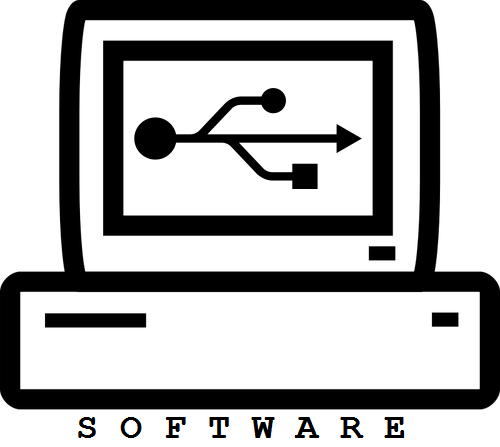
\includegraphics[width=.12\textwidth]{fig/flash-tool}
                        & 
\includegraphics[width=.12\textwidth]{fig/frog-tool}
                            \\ \hline
            Представления (код, формат)
                & 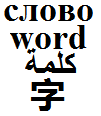
\includegraphics[width=.12\textwidth]{fig/book-code}
                    & 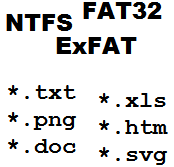
\includegraphics[width=.12\textwidth]{fig/flash-code}
                        & 
\includegraphics[width=.12\textwidth]{fig/frog-code}
                            \\ \hline
            Семантики (понимания)
                & 
\includegraphics[width=.10\textwidth]{fig/eurika}
                    & 
\includegraphics[width=.10\textwidth]{fig/eurika}
                        & 
\includegraphics[width=.10\textwidth]{fig/eurika}
                            \\ \hline
        \end{tabular}
    \end{center}
    
\end{frame}


\begin{frame}
    \frametitle{Реализация угроз (атаки) на различных уровнях доступа}
    \framesubtitle{Задание}
    
    \begin{table}[ht]
        \mode<article>{\caption{Реализация угроз на различных уровнях доступа}}
        \label{t:threatByLevelsTask}
        \centering
        \begin{tabular}[c]{|l|c|c|c|c|c|}
            \hline\hline
            & \multicolumn{5}{|c|}{Угрозы} \\ \hline
            
            \multicolumn{1}{|c|}{Уровень доступа} & 
                \rotatebox{90}{Раскрытия параметров} &
                    \rotatebox{90}{Конфиденциальности} &
                        \rotatebox{90}{Целостности} &
                            \rotatebox{90}{Доступности} &
                                \rotatebox{90}{Принадлежности} 
                                    \\ \hline
                            
                            
            Носителя                & ? & ? & ? & ? & ? \\ \hline
            Средств взаимодействия  & ? & ? & ? & ? & ? \\ \hline
            Представления           & ? & ? & ? & ? & ? \\ \hline
            Содержания              & ? & ? & ? & ? & ? \\ \hline
        \end{tabular}
    \end{table}
\end{frame}

Данные для заполнения таблицы \ref{t:threatByLevelsTask} представлены в таблицах 
\ref{t:discoverThreatByLevels},
\ref{t:confidThreatByLevels},
\ref{t:integrThreatByLevels},
\ref{t:accessThreatByLevels},
\ref{t:ownerThreatByLevels} с разбивкой по уровням доступа.

Рассмотрим реализацию фундаментальных угроз информации на разных уровнях доступа к ней. 
\begin{table}[ht]
    \caption{Реализация угрозы раскрытия параметров по уровням доступа}
    \label{t:discoverThreatByLevels}
    \centering
    \begin{tabular}[c]{|p{0.3\textwidth}|p{0.7\textwidth}|}
        \hline\hline
        Уровень доступа & 
            Реализациия угрозы раскрытия параметров\\ \hline\hline
            
        Носителя & 
            Определение типа носителя, его параметров\\ \hline
            
        Средств взаимодействия с носителем & 
            Определение способа (средств) взаимодействия с носителем. 
            Протоколы взаимодействия, среды, системы защиты\\ \hline
            
        Представления & 
            Определение способа представления. Язык, структуры данных\\ \hline
            
        Содержания & 
            Определение содержания на качественном уровне. Тематика\\ \hline
    \end{tabular}
\end{table}


\begin{table}[ht]
    \caption{Реализация угрозы конфиденциальности по уровням доступа}
    \label{t:confidThreatByLevels}
    \centering
    \begin{tabular}[c]{|p{0.3\textwidth}|p{0.7\textwidth}|}
        \hline\hline
        Уровень доступа&Реализациия угрозы конфиденциальности\\ \hline\hline
        Носителя & Кража\\ \hline
        Средств взаимодействия с носителем & Несанкционированный доступ к средствам взаимодействия\\ \hline
        Представления & Раскрытие представления. Дешифрование, декодирование, интерпретация\\ \hline
        Содержания & Раскрытие содержания. Понимание\\ \hline
    \end{tabular}
\end{table}


\begin{table}[ht]
    \caption{Реализация угрозы целостности по уровням доступа}
    \label{t:integrThreatByLevels}
    \centering
    \begin{tabular}[c]{|p{0.3\textwidth}|p{0.7\textwidth}|}
        \hline\hline
        Уровень доступа & Реализациия угрозы целостности\\ \hline\hline
        Носителя & Разрушение, уничтожение носителя\\ \hline
        Средств взаимодействия с носителем & Внедрение в средства взаимодействия\\ \hline
        Представления & Искажение данных, предложений языка\\ \hline
        Содержания & Дезинформация, ложь, обман\\ \hline
    \end{tabular}
\end{table}

\begin{table}[ht]
    \caption{Реализация угрозы доступности по уровням доступа}
    \label{t:accessThreatByLevels}
    \centering
    \begin{tabular}[c]{|p{0.3\textwidth}|p{0.7\textwidth}|}
        \hline\hline
        Уровень доступа &
            Реализациия угрозы доступности\\ \hline\hline
        Носителя & 
            Выведение из строя\\ \hline
        Средств взаимодействия с носителем & 
            Блокировка средств взаимодействия\\ \hline
        Представления & 
            Искажение метаданных, искажение соответствия структуры и 
            семантики данных. Искажение языка\\ \hline
        Содержания & 
            Запрет, обход запрета, разрушение тезауруса получателя\\ \hline
    \end{tabular}
\end{table}


\begin{table}[ht]
    \caption{Реализация угрозы принадлежности по уровням доступа}
    \label{t:ownerThreatByLevels}
    \centering
    \begin{tabular}[c]{|p{0.3\textwidth}|p{0.7\textwidth}|}
        \hline\hline
        Уровень доступа &
            Реализациия угрозы принадлежности\\ \hline\hline
        Носителя & 
            Кража, подмена идентификаторов носителей\\ \hline
        Средств взаимодействия с носителем & 
            Нарушение правил доступа, обход системы защиты, 
            блокирование подтверждений или сообщений об ошибках\\ \hline
        Представления & 
            Подделка отметок принадлежности. Например кодов 
            аутентификации MAC или цифровых подписей\\ \hline
        Содержания & Введение в заблуждение относительно происхождения 
        сведений (авторства). Плагиат. Нарушение авторских прав (право на имя)\\ \hline
    \end{tabular}
\end{table}


Отдельной областью знаний являются методы \emph{социальной инженерии}, активно использующие  человеческий фактор (психологические приемы воздействия на человека, обман, вхождение в доверие, и пр.) для получения интересующей информации. Единственным методом борьбы является обучение пользователей правилам противодействия психологическим атакам.


\subsection{Примеры конкретных атак}


\begin{frame}
    \frametitle{Некоторые виды атак}
    
    \begin{itemize}
        \item Отказ в обслуживании (Denial of service (DoS), Distibuted DoS (DDoS)).
        \item Спуфинг (Spoofing).
        \item Fishing.
        \item Человек посередине (Man-in-the-middle).
        \item Обход аутентификации.
        \item Воспроизведение.
        \item XSS.\mode<article>{
            Cross Site Scripting --- межсайтовый скриптинг. Атакуется клиент. Используется узязвимость на сервере для внедрения скриптов в web-страницу. Переходя по ссылке, сформированной злоумышленником, пользователь оказывается на странице с внедренным скриптом, который может извлекать, например инедтификаторы сессий, или устраивать DoS-атаку.
        }
        \item SQL-injection.
        \item Переполнение буфера.
        \item Целочисленные переполнения.
        \item Вирусы.
    \end{itemize}
\end{frame}


\section{Злоумышленник}


\subsection{Модели злоумышленника и побудительные мотивы}

Побудительные мотивы: корысть, любопытство, самоутверждение.

\begin{frame}
    \frametitle{Модели злоумышленника и побудительные мотивы}
    
    \begin{itemize}
        \item Инсайдер (внутренний пользователь).
        \item Хакер (любопытство, амбиции).
        \item Кракер (коммерческая выгода).
        \item Script Kiddie (незкая квалификация, самоутверждение).
        \item Шпион (промышленный, коммерческий и военный шпионаж).
        \item Уполномоченный эксперт (моделирование угроз в рамках трудовой деятельности).
    \end{itemize}
\end{frame}


\appendix


\section{Вопросы для самопроверки}


\begin{frame}[allowframebreaks]
    \frametitle{Вопросы для самопроверки}

    \begin{enumerate}
        \item Что возникает раньше: угроза или атака?
        \item{} <<Переполнение буфера>> --- это угроза или атака?
        \item В чем разница между субъектом и объектом информационной системы?
        \item Назовите фундаментальные угрозы информационной системе.
        \item Назовите первичные угрозы информационной системе.
        \item Назовите базовые угрозы информационной системе.
        \item Приведите примеры на следующие характеристики угроз:
        \begin{enumerate}
            \item Природа возникновения.
            \item Степень преднамеренности появления.
            \item Источник.
            \item Положение источника.
            \item Степень зависимости от активности ИС.
            \item Степень воздействия на ИС.
            \item Способ доступа к ресурсам.
            \item Место расположения информации.
        \end{enumerate}
        \item Назовите уровни доступа к информации.
        \item Каким образом можно реализовать угрозу принадлежности на всех уровнях доступа к информации?
        \item Для каких категорий злоумышленников материальная выгода не является главным побудительным фактором?
        \item Какие категории злоумышленников представляют наибольшую опасность для:
        \begin{enumerate}
            \item конкурентоспособности предприятия на рынке в долгосрочной перспективе;
            \item потребителя услуг предприятия в отдельно взятый момент времени;
            \item нецелевого использования ресурсов ИС предприятия;
            \item раскрытия параметров ИС предприятия?
        \end{enumerate}
        По 1-3 категории в порядке убывания опасности.
    \end{enumerate}
\end{frame}


\section{Источники}

\begin{frame}
    \frametitle{Источники}
    
    Классификация угроз представлена в \cite{bib:shangin:protect,bib:chmora:crypto,bib:yaroch:infsec}. В качестве дополнительного чтения рекомендовано ознакомится с таксономией угроз, представленной в \cite{bib:zegzda:secbase} а также обратится к главе безопасность в \cite{bib:tannen:os}.
\end{frame}


\section{Библиография}

%слайд раскладывается на несколько: allowframebreaks
\begin{frame}[allowframebreaks]{Библиография}
    \bibliographystyle{gost780u}
    \bibliography{./../bibliobase}
\end{frame}




\end{document}